\documentclass[a4paper,11pt]{article}
\usepackage[utf8x]{inputenc}
\usepackage{fullpage}
\usepackage[hyphens]{url}
\usepackage{hyperref} %this messes up the line breaks of url
\usepackage{xspace}
\usepackage{listings}
\usepackage{graphicx}
\setlength{\parindent}{0pt} 
\setlength{\parskip}{2ex}

% Title Page
\title{QRSim Tutorial Exercises}
\author{{CompLACS} boot camp\\UCL 21-22 June 2012}
\date{}

\newcommand{\sname}{QRSim\xspace}
\newcommand{\snamettt}{\texttt{QRSim}\xspace}
\newcommand{\webrepo}{\url{http://complacs.cs.ucl.ac.uk/complacs/simulator/qrsim-lastStable.zip}\xspace}

\begin{document}
\maketitle
\section*{Exercise 0:\\Installing QRSim and testing the installation}

\begin{itemize}
 \item download QRSim from \\\webrepo
 \item unzip the archive in a directory of your choice
 \item start Matlab and navigate to the directory in which the QRSim archive was unpacked
 \item in the Matlab console, add the \texttt{sim} directory to path and run \texttt{example/main.m}:\\
  \texttt{\\
  >> addpath sim\\
  >> cd example\\
  >> main}
\end{itemize}
\begin{figure}[!b]
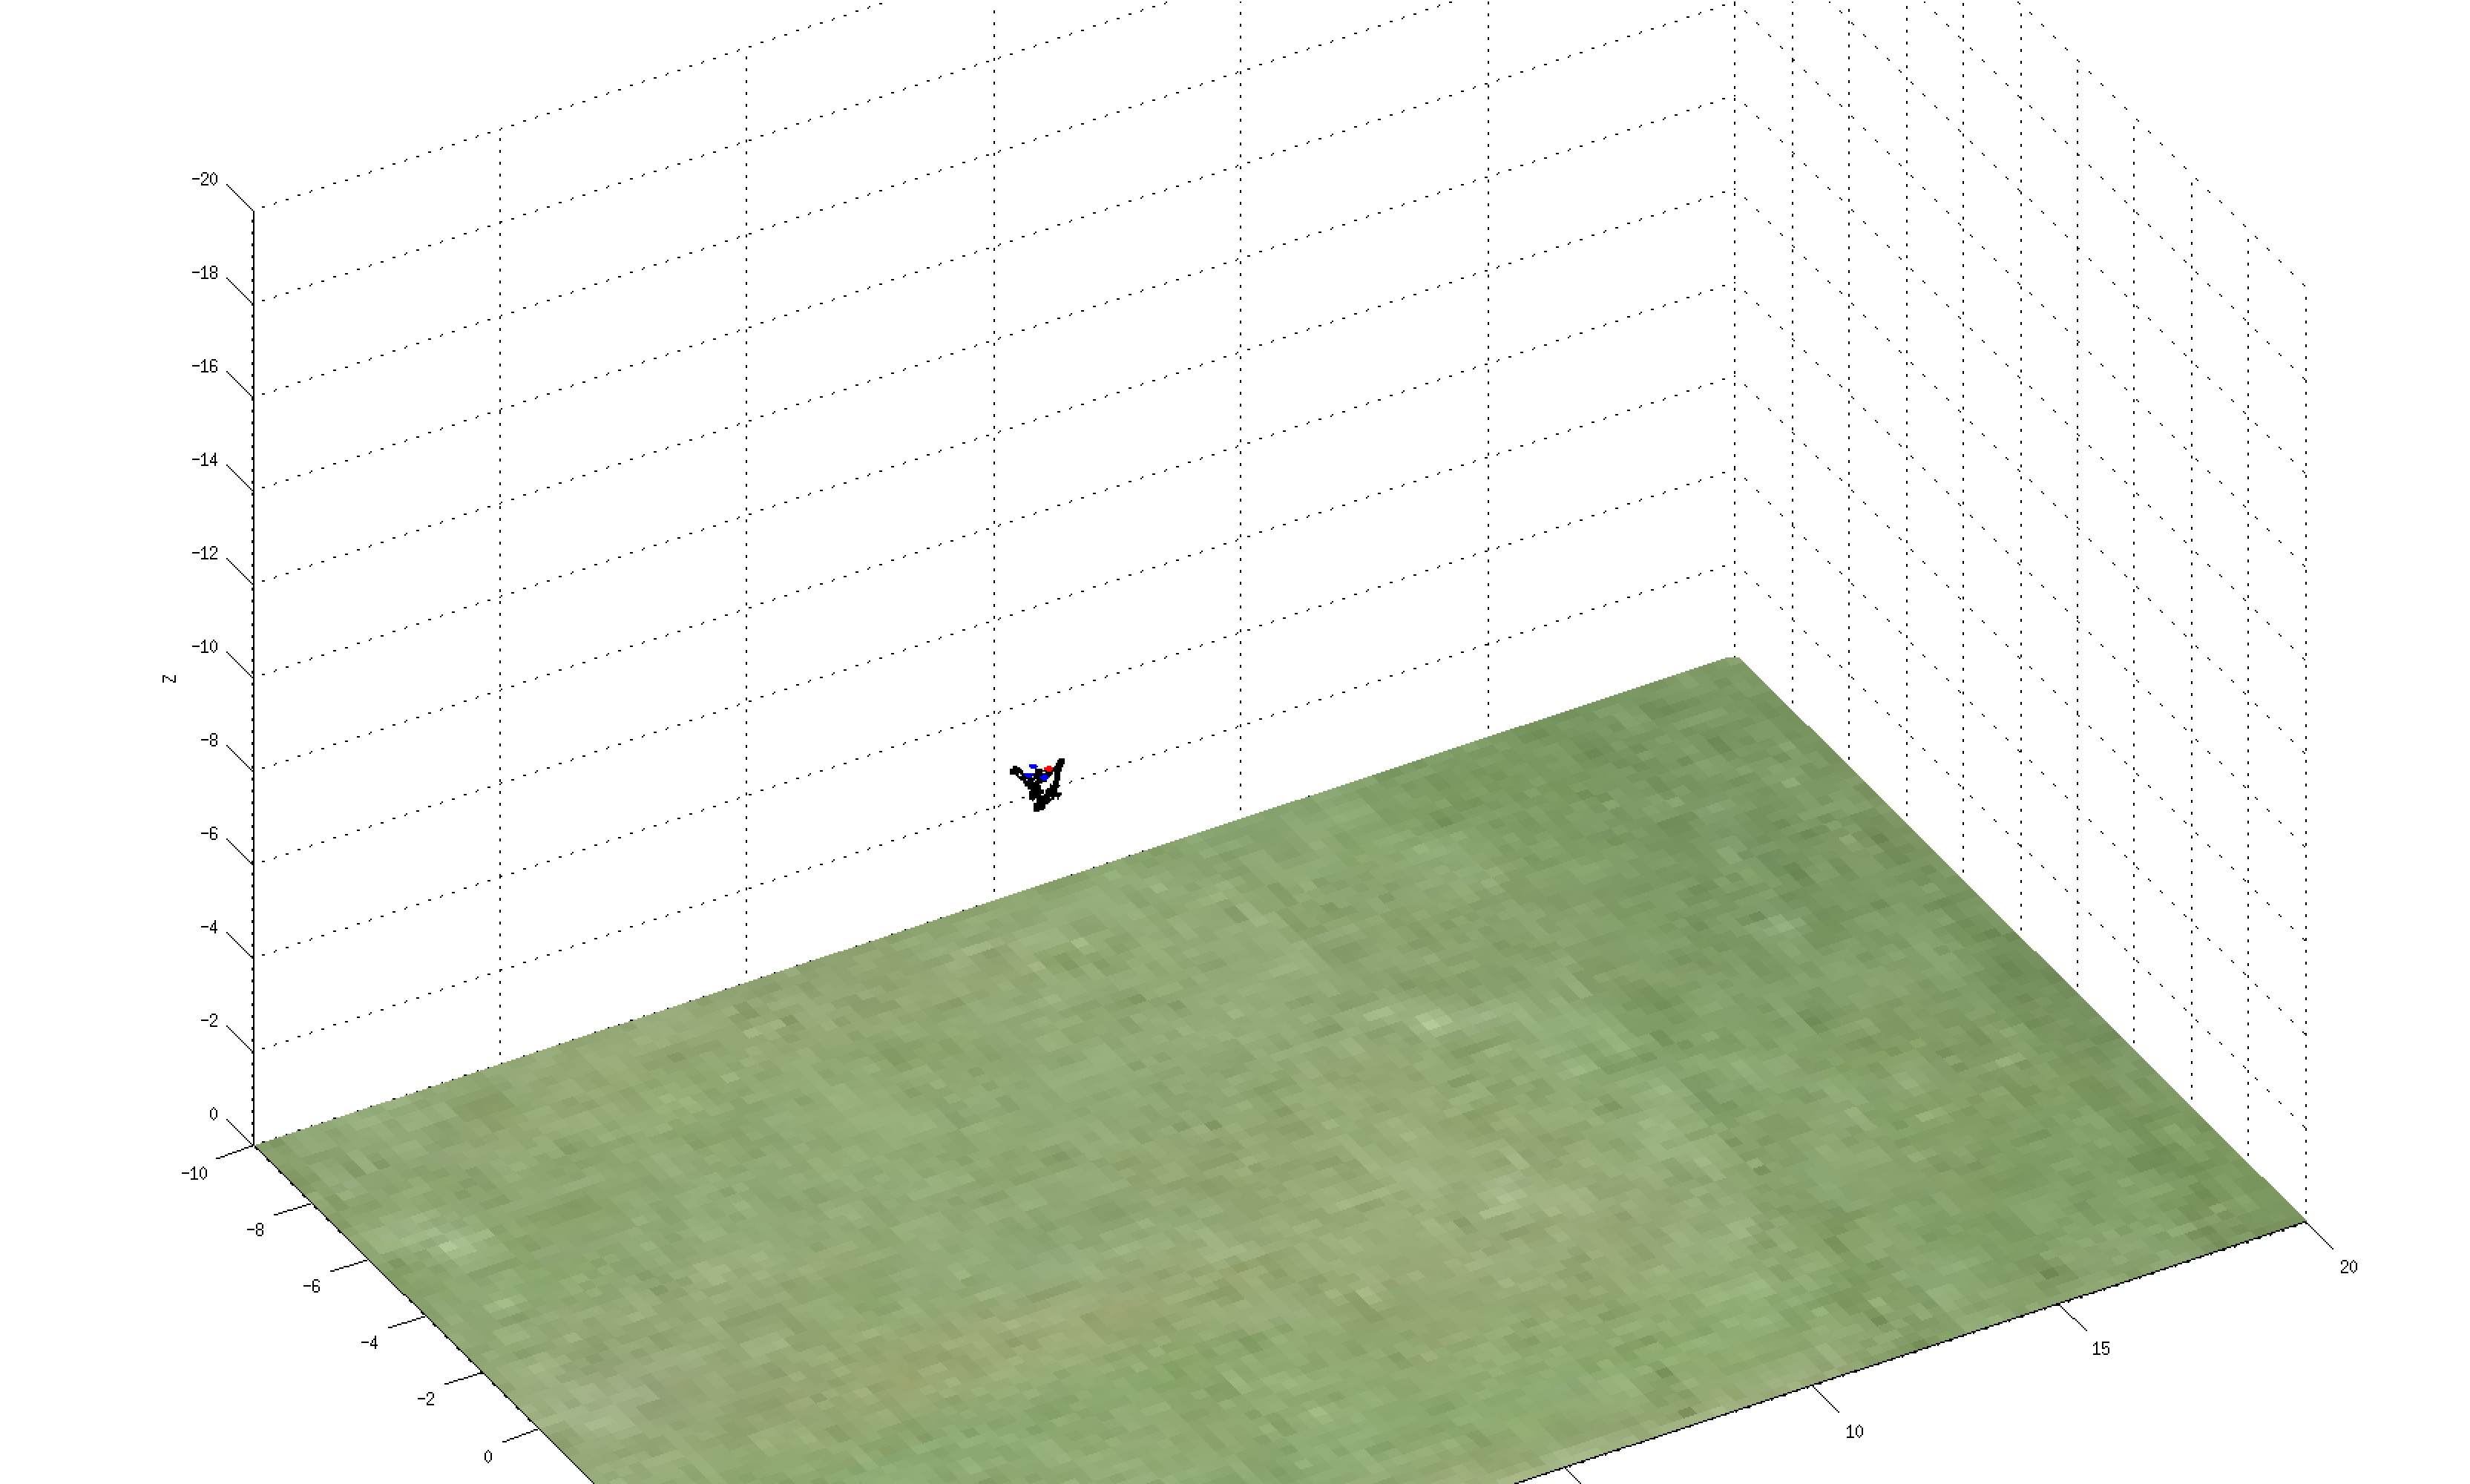
\includegraphics[width=13cm]{main.eps}
 \caption{Typical figure at the end of the run.\label{fig:main}}
\end{figure}
If the simulator is working correctly a Matlab figure (see figure \ref{fig:main}) should appear and you should see a helicopter moving about. In this task the helicopter is attempting to maintain the position it had at the start of the run, due to air turbulence and estimation error the UAV tends to drift and therefore corrective actions are needed from time to time. 

\section*{Exercise 1:\\Creating a new project}

A new qrsim simulation is usually composed of at least three files:
\begin{itemize}
 \item a main scripts that control the execution of the simulation;
 \item a task file that define the configuration for the environment objects;
 \item a platform configuration file that defines the setting for the platform sensors.
\end{itemize}
Create a new directory in a location of your choice\footnote{Using QRSim within a project only requires to have the \texttt{sim} directory in the Matlab path therefore you have complete freedom in choosing where to keep your projects.} and copy into it the files:
\begin{itemize}
 \item \texttt{example/main.m}
 \item \texttt{sim/tasks/TaskKeepSpot.m}
 \item \texttt{sim/platforms/pelican\_config.m}
\end{itemize}
Since we will be modifying these files in the following exercises it makes sense to rename them to something more meaningful; let's rename \texttt{TaskKeepSpot.m} to \texttt{TaskTutorial.m} and \texttt{pelican\_config.m} to \texttt{pelican\_config\_tutorial.m}.

Of course now we need to update the files that reference such scripts, this will give us the chance to see what references what, within one of our projects.
We start by editing \texttt{main.m} in the following way:
\begin{itemize}
 \item line 8: update \texttt{addpath(['..',filesep,'sim:..',filesep,'controllers']);} to point to the directories \texttt{sim} and \texttt{controllers} in your machine. Note that this is the only command needed to make use of QRSim in your project (this is akin to the need of including a toolbox in the Matlab path).
 \item line 14: update \texttt{state = qrsim.init('TaskKeepSpot');} to reference the renamed task \texttt{TaskTutorial.m}. Note that this is the only location in which a task is referenced.
\end{itemize}  
Now, since \texttt{TaskTutorial.m} is a Matlab class, its file name needs to match the class name\footnote{If you are not familiar with object-oriented programming in Matlab you can find more informations at \url{http://www.mathworks.co.uk/help/techdoc/matlab_oop/ug_intropage.html}}. We therefore need to open \texttt{TaskTutorial.m} in the file editor and do the following:
\begin{itemize}
 \item line 1: replace \texttt{classdef TaskKeepSpot<Task} with \texttt{classdef TaskTutorial<Task}
 \item line 28: replace \texttt{obj = TaskKeepSpot(state)} with \texttt{obj = TaskTutorial(state)}.
\end{itemize}
Finally if we look at the bottom of the method \texttt{init()} defined in \texttt{TaskTutorial.m} (line 102) we can see that the script \texttt{pelican\_config} is indicated as the configuration file that should be used for platform 1. Obviously we want to change this to \texttt{pelican\_config\_tutorial} so that the configuration file that we have in the current directory is used instead.

At this point, we have a new project completely independent from the original one we started from. You can now test that the modifications we just applied did not break the project; simply run \texttt{main} from within your project directory and you should see the same output you got for Exercise 0. 


\section*{Exercise 2:\\Familiarize with \texttt{QRSim} and platforms objects}

We now have a look in more detail at the file \texttt{main.m}; open it in your Matlab editor. 
This script implements what is possibly the simplest way of running a simulation using QRSim; nevertheless it shows the three fundamental steps that are always needed when running a simulation:
\begin{itemize}
 \item line 11: \texttt{qrsim = QRSim()}  creation of a simulation object; \\
  this instruction takes care of initializing the path variables correctly and creates (but does not initialize) the data structure that maintains the simulation state. 
 \item line 14: \texttt{state = qrsim.init('TaskTutorial')} initialization of the simulation;\\
  the setting specified in the task are used to instantiate the required platform and environment objects, and subsequently to initialize them to the starting state. After calling \texttt{init} the simulator is in a valid state and the simulation time \texttt{state.t} is equal to zero.
 \item line 35: \texttt{qrsim.step(U)} stepping the simulator;\\
 this command first updates the environment objects and then calls the function \texttt{step(U)} of the task to transform \texttt{U} into the input for each of the platforms. We will see later that in the task \texttt{TaskTutorial} the function \texttt{step(U)} does not modify the input matrix \texttt{U}; \texttt{U} is therefore expected to be already a matrix in which each column corresponds to the control inputs for a platform\footnote{Use \texttt{doc Pelican} to see details about meaning and ranges of the control inputs.}. At completion the simulation time had advanced of \texttt{state.DT}.  
\end{itemize}
From the description just given one can understand that calling \texttt{step()} only makes sense after the simulation is created and initialized to a valid state. 
In our \texttt{main.m} script the simulator is stepped within a for loop since we want to run the task for \texttt{N} steps but it is rather obvious that this does not always need to be the case. Once the simulation object is initialized the step method can be called in whatever fashion is more convenient to the user.

The control input \texttt{U} passed to the step function are computed using a PID controller, while we will look more in detail at this type of controller in Exercise 5 now we want to highlight how the controller uses the current platform estimated state retrieved using the function \texttt{state.platforms{1}.getEX()}.
This is not the only method exposed by the class \texttt{Pelican} to access the platform state we also have:
\begin{itemize}
 \item \texttt{getX()} returns the true state (noiseless) state;
 \item \texttt{getEXasX()} returns the estimated state (noisy) formatted as the noiseless state;
 \item \texttt{isValid()} returns true if the state is valid; the state can become not valid if the UAV exits the flying area (e.g. hits the ground) or if two UAVs collide.
\end{itemize}
You cans use the command \texttt{doc Pelican} to have more details about the format of the returned data\footnote{The commands \texttt{getEX(), getX()} and \texttt{getEXasX()} all accept intervals as argument (e.g. \texttt{getEX(1:3)}); this provides an easy way to query only for the variables of interest.}.
 
Now that is more clear what the \texttt{main.m} script is doing, modify it in order to produce a time plot of the true and of the estimated platform position. Use a 3 by 1 \texttt{subplot} so that you can plot each of the three (x,y,z) components independently.   
In a real platform the altitude estimated using the barometric altimeter is often more accurate than the one produced by the GPS receiver for this reason you will plot the former instead of $p_x$ in your plots.
Once you obtained the plots have a good look at the true and estimated variables, what do you notice?

\textsf{Note:}
in order to update the figure containing the 3D visualization the simulator needs to redefine the current window, this might interfere with your plot.
In order to avoid that you can store the handles of your plots before the beginning of the for loop and then update the plot inside the loop by setting the \texttt{YData} property of each plot.

\section*{Exercise 3:\\Modify task and platform settings}

So far we kept unchanged the settings of both the environment and of the platforms in our task, in this exercise we will explore the effects of changing such parameters.

Open the file \texttt{TaskTutorial.m} and look at the function \texttt{init()}, you will see that the parameters are divided into sections corresponding to the various environment objects. Also note how we use a nested naming scheme in order to specify the properties of each object.
Most of the objects have the property '\texttt{on}' which allows to enable or disable the object in question and some have a parameter \texttt{dt} that defines the update rate.

Try out some of the following changes \textsf{in turn}, and look at the resulting behavior of the helicopter (remember to save the task file before re-running \texttt{main.m}): 
\begin{itemize}
 \item set \texttt{taskparams.seed} to a number different from $0$ and run the simulation twice. What do you notice about the flight path of the helicopter?
 \item set \texttt{taskparams.display3d.on} to $0$; the simulation will run without 3D display. Did you notice any change in simulation speed?
 \item change the values of \texttt{taskparams.environment.area.limits}, you will see the 3D area changing accordingly\footnote{If you change the area so that the starting position of the helicopter is outside the flying volume the simulation won't run!}.
 \item try to set \texttt{taskparams.environment.gpsspacesegment.on} to $0$, what happens? We will see later why this is the case.
 \item set \texttt{taskparams.environment.wind.on} to $1$, and run the simulation twice with different values of \texttt{taskparams.environment.wind.direction}. You should see a clear effect on the helicopter flight pattern.
\end{itemize}

Try now to experiment with different initial values for the platform state by modifying the line \texttt{obj.simState.platforms{1}.setX([6;-8;-9;0;0;0]);} in the function \texttt{reset()} of the task. Note that you can also define the initial velocities by specifying an initial state of length 12.

Let's now continue by experimenting with the platform settings and therefore editing the file \texttt{pelican\_config\_tutorial.m}.
Immediately one can see that the file uses the same naming convention that we have seen for the environment object parameters. 
Even in this case is instructive to make changes to the setting and compare the output of the simulator. We suggest to try some of the following:
\begin{itemize}
 \item set \texttt{sensors.gpsreceiver.on} to $0$ and run the simulation; the GPS receiver noise is now off. What happens to the plots of estimated and true position that we set up in Exercise 2?
\item if now you now go back to \texttt{TaskTutorial} (maintaining \texttt{sensors.gpsreceiver.on} to $0$) and retry setting \texttt{environment.gpsspacesegment.on} to $0$; you should now be able to run the simulations without any error.
\item set \texttt{sensors.ahars.on} to $0$ to turn off any noise in the inertial sensors; this should be clearly visible if you add to the plot of Exercise 2 the true and estimated angles (or angular velocities). 
\item set \texttt{aerodynamicturbulence.on} to $0$; is the flight behavior changed?
\item set \texttt{aerodynamicturbulence.on} and \texttt{sensors.gpsreceiver.on} both to $0$; do you see a drastic improvement in the capability of the helicopter in keeping station?
\item set \texttt{dynNoise = [0;0;0;0;0;0]} and all \texttt{gpsreceiver.on} \texttt{ahars.on} \texttt{aerodynamicturbulence.on} to $0$; verify that the behavior of the simulator is now completely deterministic.
\end{itemize}

Lastly, take a look at the function \texttt{step(U)} of the task. In this case the input matrix \texttt{U} is simply returned unchanged, but in certain tasks it might be useful to do some computation within this function. For instance if we wanted a task that accepts inputs in terms of waypoints, we could have included the PID controllers computations in this function so to perform the translation from waypoints to platform controls.

\section*{Exercise 4:\\Set and reset the platform state}

We have seen how changing the initial platform state in the \texttt{pelican\_config\_tutorial.m} is very straightforward but is often necessary to be able to save, set and reset the platform state at runtime.
The platform objects expose a set of methods designed to make setting and resetting of the state very easy:
\begin{itemize}
\item \texttt{state.platforms{1}.getX()}, returns the true platform state. We have seen this method already, saving a state is simply a matter of storing the returned state in an appropriate variable.
\item \texttt{state.platforms{1}.setX(X)}, set the true platform state to the passed value. Note that in addition to overwriting the object's state this call also make sure that any other internal variable (e.g. noise model states) is appropriately set/reset. In this way running the platform forward in time will produce a state trajectory statistically independent from the ones previously obtained (even in the presence of the same control) unless the user specified a fix seed for the pseudorandom number generator.
\end{itemize}

The main QRSim object also exposes a reset method 
\begin{itemize}
\item \texttt{qrsim.reset()} resets the simulator to the initial state specified by the task. This also resets the task reward to zero, and calls the method \texttt{reset()} of the task which re-initializes the platforms state. 
\end{itemize}

With those concepts clear in mind modify \texttt{main.m} as follows:
\begin{itemize}
\item remove the \texttt{WaypointPID} controller, and replace the computation of \texttt{U} with a constant input (something like \texttt{[0;0.02;0.595;0;12]} should do);
\item modify the for loop to run the simulation for 100 time steps and save the final platform true state;
\item add a second loop to run the simulation for another 100 time steps (while storing both the true and estimated state)
\item set the platform state back to the saved state
\item add a third loop to run the simulation yet again for 100 time steps (while storing both the true and estimated state)
\end{itemize}
What do you see if you compare the state trajectory of the first run with the one of the second run? 

Now edit the file \texttt{TaskTutorial} and set the parameter \texttt{taskparams.seed} to something other than zero. 
What do you see if you re-run the code you wrote above and you compare again the state trajectory of the first run with the one of the second run? 


\section*{Exercise 5:\\Using predefined PID controllers}

In addition to accepting low level control inputs inputs (pitch and roll angles, yaw velocity and throttle) the Pelican quadrotors in use at UCL can run on-board one of two types of PID controllers. These allow them to accept inputs in the form of GPS way-point and (global frame) velocity commands. 
To replicate this capability within QRSim we also provide two of such controllers\footnote{We need to stress that since the manufacturer does not publish details about the helicopters firmware we have to consider such controllers as qualitatively but not quantitatively correct.}, they can be found in the directory \texttt{controllers}:
\begin{itemize}
\item \texttt{WaypointPID}, controller that computes the pitch, roll and throttle input necessary to achieve a desired 3D (NED) position in global frame while maintaining a specified heading.
\item \texttt{VelocityPID}, controller that computes the pitch, roll and throttle input necessary to maintain a desired velocity in global frame while keeping a specified heading.
\end{itemize}

The \texttt{WaypointPID} controller is used in \texttt{main.m} and so we have somehow used it throughout this tutorial; experiment with tasking the helicopter with different destination position by changing the way-point \texttt{wp}. To see details on the meaning of the way-point parameters use the command \texttt{doc WaypointPID} and look at the description of the method \texttt{computeU()}.   

Modify \texttt{main.m} and instead of defining a desired position (\texttt{wp}) for the helicopter to go to, define an array of desired velocity that you want the helicopter to maintain as the time progresses.
Of course you will then need to substitute the \texttt{WaypointPID}  with a \texttt{VelocityPID} and make the necessary adjustments. To see details on the meaning of the desired velocity parameters use the command \texttt{doc VelocityPID} and look at the description of the method \texttt{computeU()}.   
If you get stuck have a look at the file \texttt{example/mainVel.m} for a possible solution to this exercise.


\section*{Exercise 6:\\Defining a task reward}

A task is defined not only by the configuration of platforms and environment objects but also by the objective that needs to be achieved.
In the \texttt{TaskTutorial} class we provide two hooks for the user to define how to update and compute the cost/reward for the task:
\begin{itemize}
 \item the method \texttt{updateReward(U)} called as the last instruction of the \texttt{qrsim.step()} function. Within this function the user has access to both the current state (\texttt{obj.simState}\footnote{\texttt{obj.simState} is a handle to the simulation \texttt{state} (see Exercise 1) that is maintained within every \texttt{Task}}) result of the step update as well as to the control actions \texttt{U} that have just been executed. These can be used for instance to update a cost that is dependent on the control action, on the state or on both. 

 \item the method \texttt{reward()} called when the user executes \texttt{qrsim.reward()} on the main simulation object. Generally this function is called at the end of a task\footnote{See the call commented out in \texttt{main.m}.} and allows for instance to define an end cost for the task.
\end{itemize}
  
Although in \texttt{main.m} we use a PID controller to navigate to a way-point we can still define (and then query) a reward for the task. To do so:
\begin{itemize}
 \item uncomment the statement \texttt{qrsim.reward()} in \texttt{main.m};
 \item modify the methods \texttt{updateReward()} and \texttt{reward()} in \texttt{TaskTutorial.m} to define a reward that includes a quadratic control cost and a final cost proportional to the distance to the initial helicopter position (\texttt{obj.initialX(1:3)}).
\end{itemize}
If you get stuck you can have a look in the directory \texttt{tasks}, the file \texttt{TaskKeepSpotWithReward.m} shows a possible solution to this exercise.

Finally, we want to point out that while defining rewards within a task is very handy, this is by no means something necessary to perform simulations using QRSim. In facts the \texttt{updateReward()} and \texttt{reward()} methods of a task can simply be left empty if not needed.

\section*{Exercise 7:\\Working with several helicopters}

Up until now we only considered one single helicopter, however QRSim can readily deal with more than one platform.
Let's try to modify the task file and \texttt{main.m} to handle 10 different helicopters; to do so you will need to:
\begin{itemize}
 \item modify \texttt{TaskTutorial.m} to define a \texttt{configfile} for each of the platforms and modify the \texttt{seset()} function to define the initial state of each platform. You can easily do this with a for loop but make sure that the initial position of the platforms are sufficiently far apart otherwise they would be deemed in collision and the simulation will fail to start.
\item modify \texttt{main.m} so that ten different way-points and ten different PID controllers are created instead of only one of each. In the \texttt{for} loop use each of the ten PIDs to compute the control input for the respective helicopter. Remember to bundle up the control commands of each platform as columns of the matrix \texttt{U} so you can pass it to \texttt{qrsim.step(U)}.
\end{itemize}
If you get stuck you can have a look in the directory \texttt{example}, the file \texttt{main10.m} shows a possible solution to this exercise.

Now that you have several helicopters in your simulation you can play around with the parameter \texttt{collisionDistance} in \texttt{pelican\_config\_tutorial.m} and verify that if two platforms are closer than the collision distance both will be deemed to have an invalid state.

\end{document}          
